\documentclass[12pt]{article}

% Packages
\usepackage[margin=1in]{geometry}
\usepackage{setspace}
\usepackage{amsmath}
\usepackage{amssymb}
\usepackage{graphicx}

% Title information
\title{Project Idea: Optimal flood policy}
\author{Daniel Jonas Schmidt}
\date{\today}

\begin{document}

\maketitle

\section{Motivation}
\begin{itemize}
    \item Households have heterogenous flood risk beliefs. Those who underestimate flood risk may not buy insurance or invest enough in private adaptation measures. A universal flood insurance mandate, which would ensure that even those who underestimate flood risk are insured, is often legally and politically infeasible.
    \item This creates a potential role for government intervention in the form of flood insurance subsidies, subsidies for private adaptation measures, disaster relief programs, or a combination of all policies.
    \item Subsidies can increase insurance and adaptation towards their socially optimal level, but with sufficient heterogeneity in beliefs, there will always be a group of households that underestimate flood risk enough to stay uninsured and under-adapted even with subsidies in place. 
    \item Disaster relief programs provide a safety net for uninsured households, but they also reduce incentives to buy flood insurance or invest in private adaptation measures. 
    \item What is the socially optimal mix of these policies in the presence of heterogeneous flood risk beliefs? Is it optimal to use all available policy instruments, or only a subset? How does optimal policy depend on the distribution of flood risk beliefs, risk aversion, and other parameters?
    \item The methodological approach I have in mind is to set up a stylized theoretical model and derive analytical results where possible. To take the model to the data, we could calibrate it or try a sufficient statistics approach.
\end{itemize}

\section{Possible starting point}
\begin{itemize}
    \item One time period
    \item Fixed budget dedicated to flood policies
    \item Insurance subsidy and disaster relief as policy instruments, no private adaptation
\end{itemize}

\subsection{Household Problem}

\begin{itemize}
    \item Wealth $w$ available for consumption
    \item Flood occurs with probability $p$
    \item Household believes flood occurs with probability $q$ 
    \item Flood causes damage $d$ and there is no misperception about damage conditional on flood occurrence
    \item Flood insurance is actuarially fair and costs $p$ per unit of coverage
    \item Government subsidizes flood insurance, so household pays $(1-s)p d$
    \item If uninsured and flood occurs, household receives disaster relief that covers a fraction $a$ of the damage
    \item If insured, expected utility is
    \[
    V_{ins}(s) = u(w - (1-s)p d)
    \]
    \item If uninsured, perceived expected utility is
    \[
    V_{perc,unins}(q,a) = (1-q)u(w) + q \, u(w - (1-a)d)
    \]
    \item However, the true expected utility if uninsured is
    \[
    V_{unins}(a) = (1-p)u(w) + p \, u(w - (1-a)d)
    \]
    \item Household buys insurance if $V_{ins}(s) > V_{perc,unins}(q,a)$
    \item The minimum subjective flood risk $q$ to buy insurance is
    \[
    q^*(s,a) = \frac{u(w) - u(w - (1-s)p d)}{u(w) - u(w - (1-a)d)}
    \]
\end{itemize}

\subsection{Government Problem}

\begin{itemize}
    \item Population with distribution of subjective flood risk $F(q)$
    \item Government has budget $B$ dedicated to flood policies
    \item Government chooses subsidy $s$ and disaster relief fraction $a$ to maximize social welfare
    \[
    S(s,a) = V_{unins}(a) \cdot F(q^*(s,a)) + V_{ins}(s) \cdot \bigl(1 - F(q^*(s,a))\bigr)
    \]
    subject to
    \[
    B = pd \bigl[ a F(q^*(s,a)) + s (1 - F(q^*(s,a))) \bigr]
    \]
\end{itemize}

\subsubsection*{First-Order Conditions of the Lagrangian}
\begin{align*}
    \frac{\partial \mathcal{L}}{\partial s} &= \underbrace{(V_{unins} - V_{ins}) \cdot f(q^*) \cdot \frac{\partial q^*}{\partial s}}_{\text{welfare effect of switching households}} + \underbrace{\frac{\partial V_{ins}}{\partial s} \cdot (1 - F(q^*))}_{\text{direct benefit to insured}} \\[8pt]
    &\quad + \lambda \, pd \Biggl[ \underbrace{-(a - s) \cdot f(q^*) \cdot \frac{\partial q^*}{\partial s}}_{\text{budget effect of switching}} - \underbrace{(1 - F(q^*))}_{\text{direct subsidy cost}} \Biggr] = 0
\end{align*}
\begin{align*}
    \frac{\partial \mathcal{L}}{\partial a} &= \underbrace{(V_{unins} - V_{ins}) \cdot f(q^*) \cdot \frac{\partial q^*}{\partial a}}_{\text{welfare effect of switching households}} + \underbrace{\frac{\partial V_{unins}}{\partial a} \cdot F(q^*)}_{\text{direct benefit to uninsured}} \\[8pt]
    &\quad + \lambda \, pd \Biggl[ \underbrace{-(a - s) \cdot f(q^*) \cdot \frac{\partial q^*}{\partial a}}_{\text{budget effect of switching}} - \underbrace{F(q^*)}_{\text{direct relief cost}} \Biggr] = 0
\end{align*}

\begin{itemize}
    \item Disaster relief $a$ and insurance subsidy $s$ cannot be negative. Thus, we also need to consider corner solutions where either $s=0$, or $a=0$.
    \item Depending on the shape of the distribution, several local optima could exist.
    \item Nevertheless, the first-order conditions nicely illustrate the role of the fraction of insured households and the density of beliefs at the margin:
    \begin{itemize}
        \item Increasing insurance subsidies $s$ is most effective when there are many households close to the margin of buying insurance relative to the number of households that is already insured.
        \item Increasing disaster relief $a$ is most effective when there are few households close to the margin of buying insurance relative to the number of households that is uninsured.
    \end{itemize}
\end{itemize}

\subsubsection*{Numerical solution}

\begin{itemize}
    \item CRRA utility with $\gamma = 2$
    \item Wealth $w = 1$, flood damage $d = 0.5$
    \item True flood probability: $p = 2\%$
    \item Government budget: $B = 0.001$ (i.e., 10\% of total expected flood damages)
    \item Belief distribution: Beta with mean $\mu_q = 1\%$ and standard deviation $\sigma_q \in \{0.5\%, 0.7\%, 1.0\%\}$
    \item The minimum subjective flood risk $q^*(0,0)$ to buy insurance without any policies is approximately 1\%
\end{itemize}

\begin{figure}[h]
\centering
\begin{minipage}{0.48\textwidth}
\centering
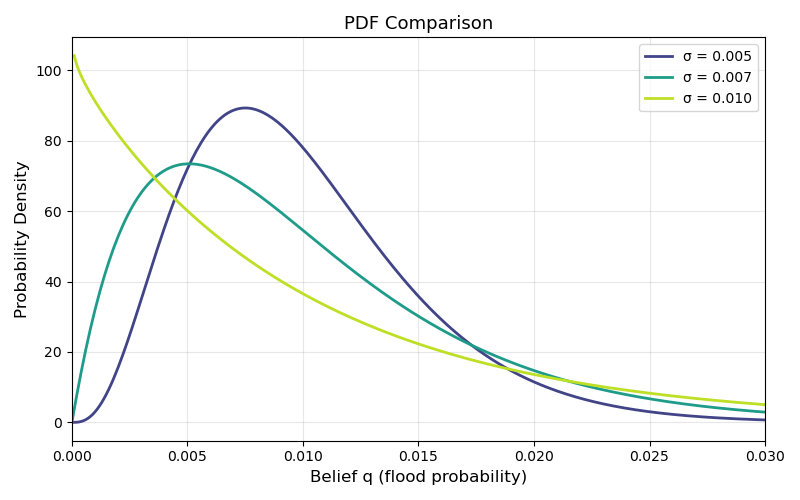
\includegraphics[width=\textwidth]{figures/pdf_comparison.png}
\caption{Distribution of subjective flood risk beliefs}
\end{minipage}
\hfill
\begin{minipage}{0.48\textwidth}
\centering
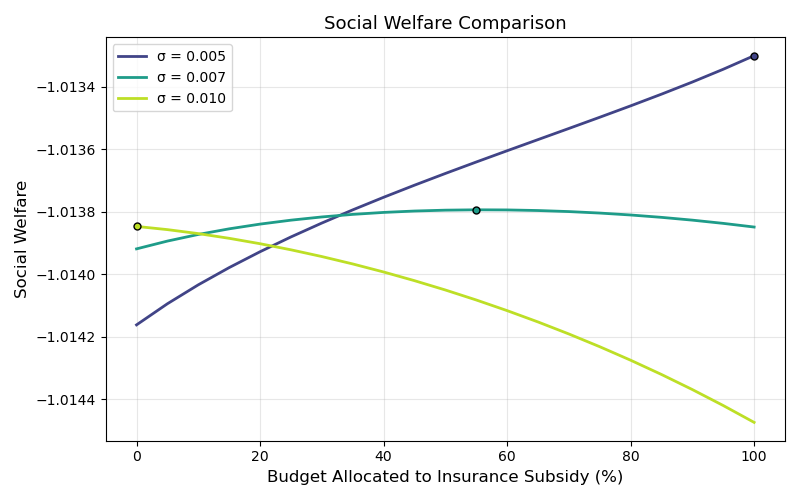
\includegraphics[width=\textwidth]{figures/welfare_comparison.png}
\caption{Social welfare as a function of budget allocation to subsidies. Dots mark optimal policy.}
\end{minipage}
\end{figure}

\begin{itemize}
    \item {Low dispersion of beliefs} ($\sigma = 0.5\%$): Insurance subsidies only ($s = 17\%$, $a = 0\%$) since many households are close to the margin of buying insurance and can be incentivized to do so through subsidies. Insurance take-up increases from 43\% to 57\%.
    \item {Medium dispersion of beliefs} ($\sigma = 0.7\%$): Mixed policy ($s = 13.9\%$, $a = 7.4\%$) so that insurance take-up stays roughly constant at 40\%.
    \item {High dispersion of beliefs} ($\sigma = 1.0\%$): Disaster relief only ($s = 0\%$, $a = 14\%$) since relatively few households are at the margin of buying insurance. Insurance take-up decreases from 37\% to 27\%.
\end{itemize}

\section{Extensions}
\subsubsection*{Natural next steps}
\begin{itemize}
    \item Introduce administration costs for flood insurance and disaster relief
    \item Include private adaptation measures
    \item What is the optimal budget dedicated to flood policies?
\end{itemize}
\subsubsection*{Possible further extensions/ Things to discuss verbally but not model formally}
\begin{itemize}
    \item Correlation of flood risk beliefs with income and/or wealth
    \item Heterogeneity in risk aversion
    \item Sorting of households into flood-prone areas based on beliefs
    \item Public adaptation measures
    \item Liquidity-provision policies (disaster loans, 401k withdrawals, mortgage relief)
    \item Government support for households in flood-prone areas creates incentives to build in flood-prone areas/ migrate to flood-prone areas
\end{itemize}

\section{Caveats}
\begin{itemize}
    \item There are no good sources of the distribution of flood risk beliefs, but this would be a key input to the model.
    \begin{itemize}
        \item The first-order conditions depend only on the fraction of insured households (publicly observable) and the density of beliefs at the margin (can potentially be recovered from the price elasticity of insurance demand). This suggests we may be able to assess whether the current policy mix is locally optimal using these two statistics alone, without full knowledge of the belief distribution.
    \end{itemize}
    \item Even the relatively simple model outlined above cannot be solved analytically for most utility functions and belief distributions.
    \begin{itemize}
        \item Can we think of an alternative modelling approach that yields more tractable results? 
    \end{itemize}
\end{itemize}

\end{document}